
\documentclass[12pt,a4paper]{article} 
\usepackage{indentfirst,latexsym,graphicx} 
\usepackage[utf8]{inputenc} % Включаем поддержку UTF8
\usepackage[russian]{babel}
\usepackage{amssymb,amsmath} 
\graphicspath{{img/}} % тут картинки твои
\usepackage[left=2cm,right=2cm,top=2cm,bottom=2cm,bindingoffset=0cm]{geometry}
\usepackage{amsmath, amssymb, amsthm}

\begin{document}

1)Чем различаются модели диода для большого и малого сигналов?
Режим малого сигнала описывает  поведение диода при малых изменения сигнала на его зажимах.
	
	Т.к. изначально диод будет иметь определенную рабочую точку, то при подаче малого сигнала она сместится на очень маленькое расстояние так, что это смещение можно будет аппроксимировать до линейного участка, а следовательно на нем можно будет использовать методы при линейных расчетах.
	
	Напротив, режим большого сигнала ассоциируется с подачей на вход большого изменения сигнала, следовательно РТ сместится на достаточное расстояние. Т.е. уровень сигнала будет влиять на положение РТ.
	
	Рассмотрим модель малого сигнала для диода:
	
	$r_b$ - объемное сопротивление базы
	\begin{center}

	\begin{figure}[h!]
		\center{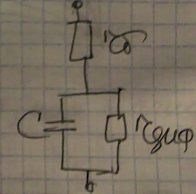
\includegraphics[scale=0.7]{1.png}}
		\caption{Модель малого сигнала для диода}	
		\label{VD1}
	\end{figure}
\end{center}
С - емкость диода

$
	C=C^u_{bar}+C^u_{dif}
$ - в зависимости от типа включения

$
\left\{
	\begin{aligned}
		C=C^u_{bar},U=U_{obr}\\  
  		C=C^u_{dif},U=U_{dif}\\
  	\end{aligned}
\right.
$

$
C^u_{bar}=C^0_{bar}\left(\frac{\psi_k}{\psi_k + U_{obr}}\right)^\frac1n
$
n=2 - резкое, n=3 - плавное

$C_{dif}=\frac{\tau(I_{ust})}{\varphi_t}=\tau\Delta$ - время жизни несновных носителей в слаболегиованной области.

$I_{ut} = I_0(exp\frac{U}{\varphi_t}-1)$ - ток утечки, который включает и теплоаой ток диода.
Модель диода для большого сигнала:
\begin{center}
\begin{figure}[h!]
		\center{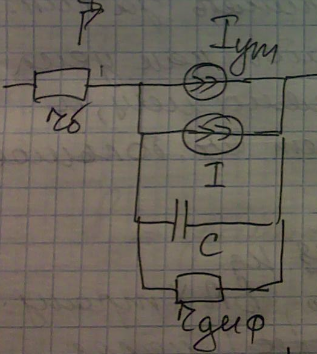
\includegraphics[scale=0.4]{2.png}}
		\caption{Модель большого сигнала для диода}	
		\label{VD3}
	\end{figure}
\end{center}	
$I=I_m(exp\frac{U}{\varphi_t}-1)$

$I_{yt}$ - ток утечки
$C=C^u_{bar}+C^u_{dif}
$
$\varphi_t=0,025B$ - темпиратурный потенциал

ВАХ Диода:
\begin{center}
\begin{figure}[h!]
		\center{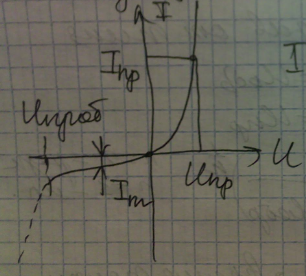
\includegraphics[scale=0.4]{3.png}}
		\caption{Вах диода}	
		\label{VAX}
	\end{figure}
\end{center}
$I_m=qS\left(\frac{D_n n_{p0}}{L_n}+\frac{D_p p_{n0}}{L_p}\right)$

Эквивалентная схема транзистора:

1)Для больших сигналов:
\begin{center}
\begin{figure}[h!]
		\center{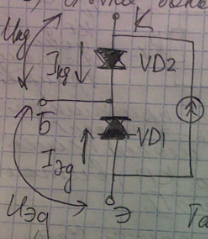
\includegraphics[scale=0.4]{4.png}}
		\caption{Эквивалентная схема диода для больших сигналов}	
		\label{ekvVD1}
	\end{figure}
\end{center}
$BI_{ed} - B_uI_{kd}$

Такая модель транзистора отражает наличие в нем 2х p-n-переходов с номерами диодов VD1 и VD2, встречновключенных.

Вз-ке(!!!!!!!не разобрал) переходов отражено с номером генератора

$I_2 = BI_{ed} - B_uI_{kd}$

Каждый из токов переходов складывается из дрейфовых и диффузионных составляющих:

$I_{ed} = I_{dif} - I_{dreif}$

$I_{dif} = I_{te}(exp(\frac{U_{ed}}{\varphi_m}))$

$I_{dreif}=I_m\Rightarrow I_{ed}=I_{te}(exp(\frac{U_{ed}}{\varphi_m}-1))$

Аналогично 
$I_{kg}=I_{mk}(exp(\frac{U_k}{\varphi_m}-1))$

Для транзисторов выполняется соотношение
$BI_{te} = B_uI_{mk}$

Рассмотрим диоды:
\begin{center}
\begin{figure}[h!]
		\center{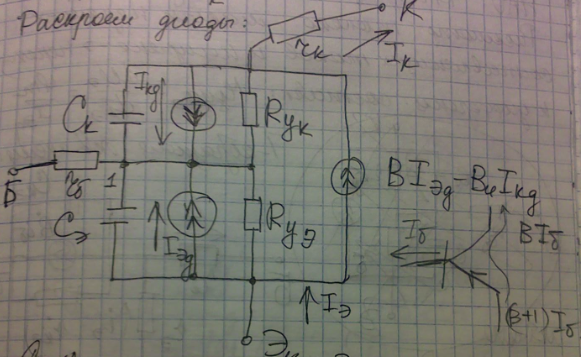
\includegraphics[scale=0.4]{5.png}}	
		\label{VD}
	\end{figure}
\end{center}
$C_k и C_e$ – емкости К и Э
Для каждого узла можно записать:

$I_{bst} = I_{ed} +\frac{U_{ed}}{R_{ye}} + I_{kd} + \frac{U_{kd}}{R_{ky}}$(узел 1)

$I_{est} = I_2 + I_{ed}  + \frac{U_{ed}}{R_{ye}}=(B+1)I_{ed} - B_u I_{kd} + \frac{U_{ed}}{R_{ye}}$

$I_{kst} = I_2 + I_{kd}  + \frac{U_{kd}}{R_{yk}}$

Модель для малого сигнала: 

НАО: КП закрыт, т.е. $I_{kd}=-I_{tk}=const$

Рассмотрим только малых переменных перем-х составляющих токов и напряжения -> переход к дифференциальной составляющей
\begin{center}
\begin{figure}[h!]
		\center{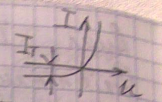
\includegraphics[scale=0.7]{vax2.png}}	
		\label{VAX2}
	\end{figure}
\end{center}

$r_{dife} = \frac{dU_{e}}{ dI_e }=\frac{\varphi_m}{ I_{ed} }$

T- образная эквивалентная схема:
\begin{center}
\begin{figure}[h!]
		\center{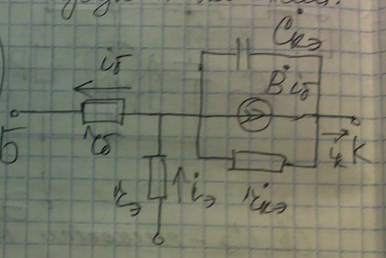
\includegraphics[scale=0.4]{T-obr.png}}	
		\label{T-obr}
	\end{figure}
\end{center}
$B=\frac{B_0}{1+j\frac{f}{f_B}}$

$f_B$ – высшая граничная частотная характеристика
частотная зависимость коэффициента усиления по току $f_B=\frac{1}{2\pi r}$
$i_{ed} = i_b - i_{ce} - i_{zk}$

$i_b$ – ток базы, $i_{ce}$ – ток через Cэ

$(i_b - i_{zk})(r_{eb}||\frac{1}{jwc_e})= i_{ce}\frac{1}{jwc_e}$(*)
\begin{center}
\begin{figure}[h!]
		\center{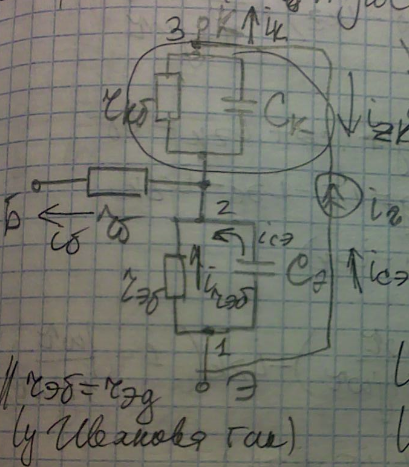
\includegraphics[scale=0.4]{10.png}}	
		\label{}
	\end{figure}
\end{center}
Связь $i_{ce}$ с $i_{cb}$(Из картинки)

$I_{ce}+i_{reb} + i_{zk}=i_b$

$I_{ce}= i_b -  i_{zk} - i_{reb}$

$U_{ce} = U12$

$U_{ce}=i_{ce}z_{ce}= i_{ce}\frac{1}{jwc_e}$

Тогда из (*):

$I_{ce} = \frac{(i_b - i_{zk})r_{eb}}{1+jwr_{ed} C_e}jwc_e$

$C_e=\frac{\tau I_e}{\varphi_t}, r_{ed}=\frac{\varphi_t }{ I_e }$

$r_{ed} C_e \approx\frac{\tau I_m}{\varphi_t }\frac{\varphi_t }{ I_e }$

тогда $i_{ce}=(i_b - i_{kz}) \frac{jw\tau}{1+ jw\tau}$

$i_2=Bi_{ed}, i_{ed}+i_{ce}+i_zk=i_b$

$i_{ed}= i_b-i_{es}-i_{zk}$

$i_2=B(i_b-i_{es}-i_zk)$

$i_2=B(i_b(1- \frac{jw\tau}{1+ jw\tau })-i_{es}-i_{zk}(1- \frac{jw\tau}{1+ jw\tau }))=B(i_b-i_{zk})$

уравнение для K, узел 3

$i_k=i_2-i_{zk}=B_0 i_{ed} - i_{zk}=Bi_b - (B+1)i_{zk}$

Из полученного уравнения:

$R_{ke} = \frac{ R_{kb} }{B+1}$

$C_{ke} = C_k(B+1)$, т.о. мы можем пренебречь $C_e$, т.к. он учитывается в B
\begin{center}
\begin{figure}[h!]
		\center{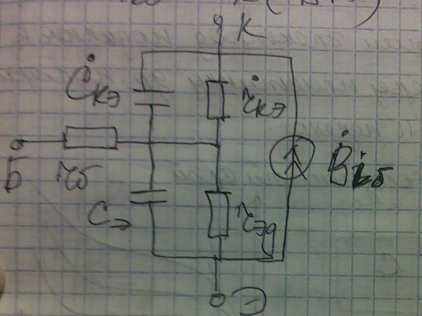
\includegraphics[scale=0.4]{11.png}}	
		\label{}
	\end{figure}
\end{center}


3)Модели для большого и малого сигнала УПТ.

Рассмотрим устройство УПТ. Также транзистор основаный на работе носителей зарядов ?? знака. Основной вид движущихся носителей -> дрейф. Работой УПТ управляет напряжение (на З-И)
Существует 2 основных вида:

1)УПТ с управляемым p-n-переходом

2)МДП 

К каналу по бокам подключены 2 электрода -> C  и U, а третий электрод подключен к области p-типа через пластинку  другой полярности. Следовательно возникает p-n-переход
\begin{center}
\begin{figure}[h!]
		\center{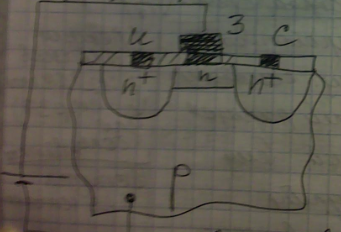
\includegraphics[scale=0.4]{mdp1.png}}	
		\label{}
	\end{figure}
\end{center}
\begin{center}
\begin{figure}[h!]
		\center{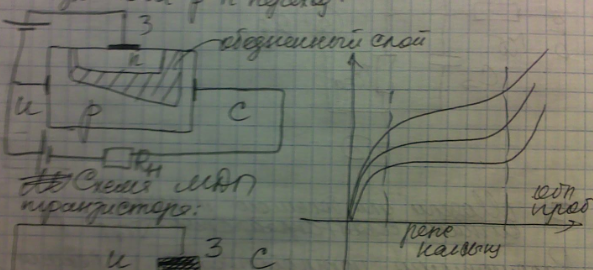
\includegraphics[scale=0.4]{mdp2.png}}	
		\label{}
	\end{figure}
\end{center}
В цепи С-И имеются 2 p-n-перехода, при чем один обязательно заряжен(???) Если $U_{zu}=0$, канал между C и  U отсутствует.

Если на 3 подать отрицательное напряжение, то приповерхностный слой обогатится дырками => тока не будет.
Если $U_{zu}>0$, то сначала образуется объединенный слой, а затем инверсионный слой e – канал.

Эквивалентная схема для больших сигналов:
\begin{center}
\begin{figure}[h!]
		\center{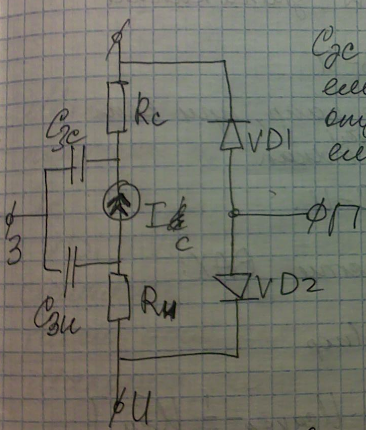
\includegraphics[scale=0.4]{mdpekv.png}}	
		\label{}
	\end{figure}
\end{center}
$C_{zc}$ и $C_{zu}$ – емкость отракс(?????????) распределенная емкость затвор-канал.

VD1 – переход U-подложка

VD2 – сток подложка

$R_u$ и $R_c$ – объемные сопротивления полупроводника.

Основная зависимость $I_c=f(U_{zu})$
\begin{center}
\begin{figure}[h!]
		\center{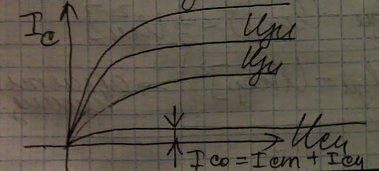
\includegraphics[scale=0.4]{mdposnzav.png}}	
		\label{}
	\end{figure}
\end{center}

На подложку подается самый высокий потенциал, что бы диоды VD1 и VD2 всегда были закрыты.

$I_c=b[(U_{zn} - U_{por})U_{cu}-\frac12 U_{cu}^2]$ – ВАХ


b – удельная крутизна
$b = \frac{\mu w}{L}$
L – длина канала
W – ширина канала

$U_{zu}$ – напряжение на З-И
$U_{por}$ – пороговое напряжение, при котором появляется канал.
$U_{cu}$ – напряжение на C-U

Для горизонтальной части ВАХ:

$U_{cunas}=U_{zn} - U_{por}$

$I_c=\frac{b}{2}[U_{zn} - U_{por}]^{2}$ – область насыщения

Из этой формулы можно получить S – крутизна

$S = b(U_{zu} - U_{por})$

S характеризует управляющее действие З на ток С

$S= \frac{\delta I_c}{\delta U_{zu}}$

$U_cu=const$

Малосигнальная эквивалентная схема может быть получена из нелинейной эквивалентной схемы на $I_c=SU_{zu}$, где $S= \frac{\delta I_c}{\delta U_{zu}}$   $U_{cu}=const$, а диоды VD1 и VD2 подменяются малосигнальными схемами.

Рассмотрим этот вариант.
Малосигнальная схема для полевых транзисторов:
\begin{center}
\begin{figure}[h!]
		\center{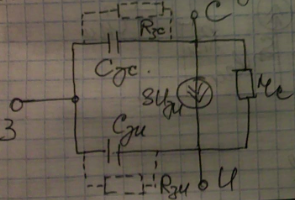
\includegraphics[scale=0.4]{polmalosign.png}}	
		\label{}
	\end{figure}
\end{center}
$R_c$ – дифференциальное сопротивление канала на пологом участке
$S - U{zn}$ – источник тока, отражающий усиленные свойства транзистора.
$R_{zu}$ и $R_{zc}$ – обратные сопротивления p-n=перехода, а $С_{zu}$ и $С_{zc}$ – барьерные емкости.

Малосигнальная схема МДП – транзистора.
\begin{center}
\begin{figure}[h!]
		\center{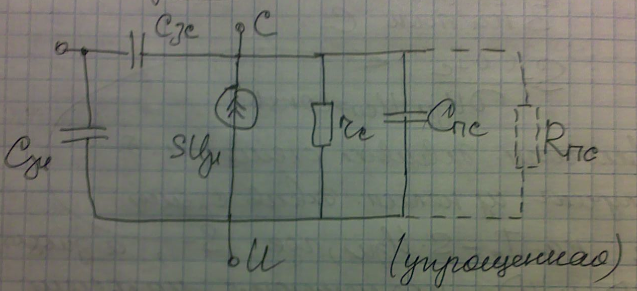
\includegraphics[scale=0.4]{mdpmalosign.png}}	
		\label{}
	\end{figure}
\end{center}
$R_{zu}$ и $R_{zc}$ – сопротивления диэлектрика затвора.

$S_{z}$ $U_{zu}$ и $S_n U_n$ – отражают усилительные способности транзисторов.
\pagebreak
\begin{center}
\begin{figure}[h!]
		\center{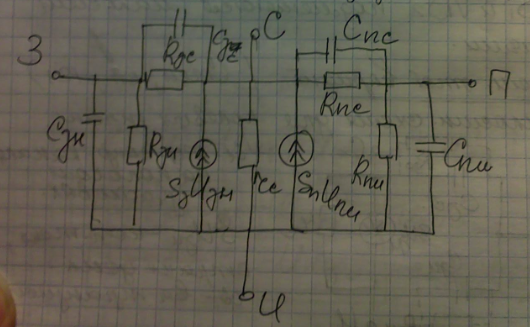
\includegraphics[scale=0.4]{mdp3.png}}	
		\label{}
	\end{figure}
\end{center}
$C_{pi}$ , $C_{ps}$ – барьерные емкости переходов.

$R_{pi}$, $R_{ps}$ – обратные сопротивления переходов.

Малосигнальные параметры:

Крутизна $S=\frac{dI_c}{dU_{zu}}$

$R_c = \frac{dU_{cu}}{dI_c}$

Коэффициент усиления: $K=\frac{ dU_{cu} }{dI_c}$
$K=Sr_c$
В области насыщения $S=b(U_{zu} - U_{por})$

\end{document}